\newcommand{\dagmcModel}[2] {
  \null %emptyline
  \textbf{\uppercase{#1}} 
  \begin{adjustwidth}{2.5em}{0pt}
    #2
  \end{adjustwidth}
  \null
}

\chapter{Introduction}\label{ch:introduction}

Methods for modeling radiation transport to determine particle flux, or derived
quantities, across space, angle, energy and time known as \textit{phase
  space}. The behavior of these particles is described by the linear Boltzmann
transport equation \cite{Ulam_1949}. Deterministic codes solve this transport
equation by discretizing the phase space of the problem, but time and memory
constraints often limit the resolution of phase space in practical problems.

The Monte Carlo approach to modeling Radiation transport simulates the
interaction of individual particles across phase space \cite{Lewis_1993}. This
method was developed at Los Alamos National Laboratory (LANL) during World War
II by Fermi, von Neumann, Ulam, Metropolis, and Richtmyer \cite{LANL_1987}. It
uses a random walk process to solve the transport equation. Pseudo-random
numbers are used to sample probability distribution functions representing
properties of the virtual medium and in turn determine the particle interaction
outcomes. This stochastic approach requires the simulation of many particles to
reduce the statistical uncertainty of the solution, where the uncertainty is
inversely proportional to the square root of the number of particles
simulated. As the number of simulated particles approaches infinity, tallied
quantities approach the value of the continuous solution.

The pros and cons of the deterministic and Monte Carlo approaches complement
each other. While deterministic approaches inherently calculate a solution over
the entire problem domain, they take on additional error by discretizing phase
space. In contrast, Monte Carlo methods only incur error associated with input
parameters such as cross sections or geometry specifications, but it is
challenging to achieve a global solution with uniform statistical error using
this approach. Computationally, deterministic methods typically suffer memory
and runtime costs that scale with the resolution of the discretized phase space
whereas Monte Carlo methods are typically limited by the runtime needed to
achieve satisfactory uncertainty in a region of interest.


\section{Monte Carlo Geometry}


Historically, Monte Carlo codes Constructive Solid Geometry (CSG) as their
\textit{native} geometry representation. CSG represents 3D regions of virtual
space using Boolean combinations of half spaces defined by quadratic
surfaces. To define the geometry, the surface and volume definitions are entered
into a text file. This format for geometry is robust once defined properly, but
is limited in representation compared to more modern geometric modeling tools
like Computer-Aided Design (CAD).

CAD allows for increased accuracy in model representation and better human
efficiency. CAD engines can represent higher-order surfaces and provides access
to models used for analysis in other engineering domains. These shared models
allow for a common problem domain in coupled simulations. CAD systems also
provide a rich set of tools for model generation, topological representation,
and design iteration. For highly complex, well-developed models, these tools are
more intuitive and efficient for human use over alteration of native text-based
formats. Several tools exist for converting native CSG models to and from CAD
systems. A few have the capability to perform simulations directly on CAD
geometries as well \cite{Leppanen_2015}.

The Direct Accelerated Geometry Monte Carlo (DAGMC) \cite{Tautges_2009} toolkit
is one of several software packages which enables Monte Carlo simulations on
CAD-based geometries. DAGMC's design allows it to serve as a particle tracking
and geometry kernel for a variety of Monte Carlo codes listed
in Table \ref{tab:dagmc_implementations}.

\begin{table}[H]
  \centering
  \begin{tabular}{c c}
    \hline
    Monte Carlo Code & DAGMC Implementation \\
    \hline
    MCNP5\cite{LANL_MCNP5_VOLIII}            & DAG-MCNP5            \\
    MCNP6\cite{Goorley_2016}                 & DAG-MCNP6            \\
    Fluka\cite{Bohlen_2014}                  & FluDAG               \\
    Tripoli4\cite{Malouch_2017}              & DAG-Tripoli4         \\
    Geant4\cite{GEANT4_2003}                 & DagSolid             \\
    Shift\cite{Pandya_2016}                  & DAG-Shift            \\
    \hline
  \end{tabular}
  \caption{A list of Monte Carlo codes and the names of their corresponding DAGMC implementations.}
  \label{tab:dagmc_implementations}
\end{table}

\section{Statement of Problem}\label{sec:problem-statement}

While the use of CAD geometries brings the benefits outlined above, it also adds
complexity to particle tracking during Monte Carlo simulations. Particle
crossings with higher-order surfaces are difficult and sometimes impossible to
compute analytically. One method of addressing this problem is to discretize the
analytic CAD surfaces into a triangle surface mesh. This generalizes
intersections with surfaces to intersections with a set of planar.
surfaces. However, a large number of triangles are needed to maintain an
accurate representation of surfaces throughout the model. As a result, the
costly search for surface crossings causes simulations on CAD-based geometries
to take much longer than native CSG models.

The intersection of a particle and trajectory with a triangulated surface is a
well-researched problem in the area of ray tracing. In this field, geometries
are also triangulated for visualization and rendering purposes. DAGMC currently
employs techniques from this field to accelerate geometric queries, but it is
still slower than native geometry implementations in CSG. DAGMC's simulations
are anywhere from 2.5 to 10 times longer than those of their native
counterparts.

Table \ref{dag-mcnp-benchmarks} represents a comparison of several
representative MCNP problems between the native geometry representations and
DAGMC coupled with MCNP, or DAG-MCNP. For smaller problems with simple
geometries and relatively low numbers of histories required to reach a low level
of statistical uncertainty, this might not pose as much of a problem to
users. As problem geometries become more complicated and the number of histories
becomes larger however, the difference in computing time becomes important when
run times extend to days or weeks longer than they would using the native MCNP
CSG geometry representation. These models include the Frascati Neutron Generator
(FNG), the Advanced Test Reactor (ATR), the University of Wisconsin Nuclear
Reactor (UWNR), and the neutron Time of Flight device at the Institute for
Science and International Security.

\begin{table}[H]
  \centering
  \begin{tabular}{l c c c}
    \toprule
    Model & Native ctme (min) & DAG-MCNP ctme (min) & Timing Ratio \\
    \hline
    FNG   & 5871.92           & 22769.33            & 3.9   \\
    ATR   & 901.68            & 8627.80             & 9.6   \\
    UWNR  & 8767.29           & 69429.60            & 7.9   \\
    nTOF  & 16.2              & 29.1                & 1.8   \\
    \hline
  \end{tabular}
  \caption{Table comparing the performance of DAG-MCNP to native MCNP for the
    same models after translation to a CAD-based surface mesh.}
  \label{dag-mcnp-benchmarks}  
\end{table}

As a part of this study, these runs were repeated using the profiling tool,
Callgrind \cite{Pena_2016}, to determine where computing time is being spent in
both the DAG-MCNP and native MCNP runs. Because the geometry representation and
query system is the only difference between the two models, it is expected that
the time is being spent there, but it is practical to confirm this and useful to
know more specifically where in the query system this is occurring. All
callgraphs are displayed with the MCNP \textit{history\_} subroutine at the
top. It is inside this subroutine that MCNP calls DAGMC to fulfill geometric
queries about the model. It should also be noted that only time spent simulating
particle histories is reported in Table \ref{dag-mcnp-benchmarks}, not including
setup operations for simulation such as nuclear cross section loading and
acceleration data structure construction.

In Figure \ref{dagmc-fng-coarse} a callgraph for a profiling run of FNG for 1e7
histories is provided. In this callgraph it is shown that the time spent in
transport is dominated by MOAB's ray tracing process used by DAGMC to track
particles as they move through the geometry. About 60\% of the runtime is spent
in DAGMC's \textit{ray\_fire} while in native MCNP the relative time spent on
this process is reduced to ~5\% with the majority of the time spent in
calculating cross sections under the \textit{acetot\_} subroutine.

\begin{figure}[H]
  \centering
  \caption{Callgraph of DAG-MCNP FNG run for \num{1E7} histories. (Processes taking
    $<$10\% of the runtime are filtered out in order to simplify the callgraph.)}
  \label{dagmc-fng-coarse}
  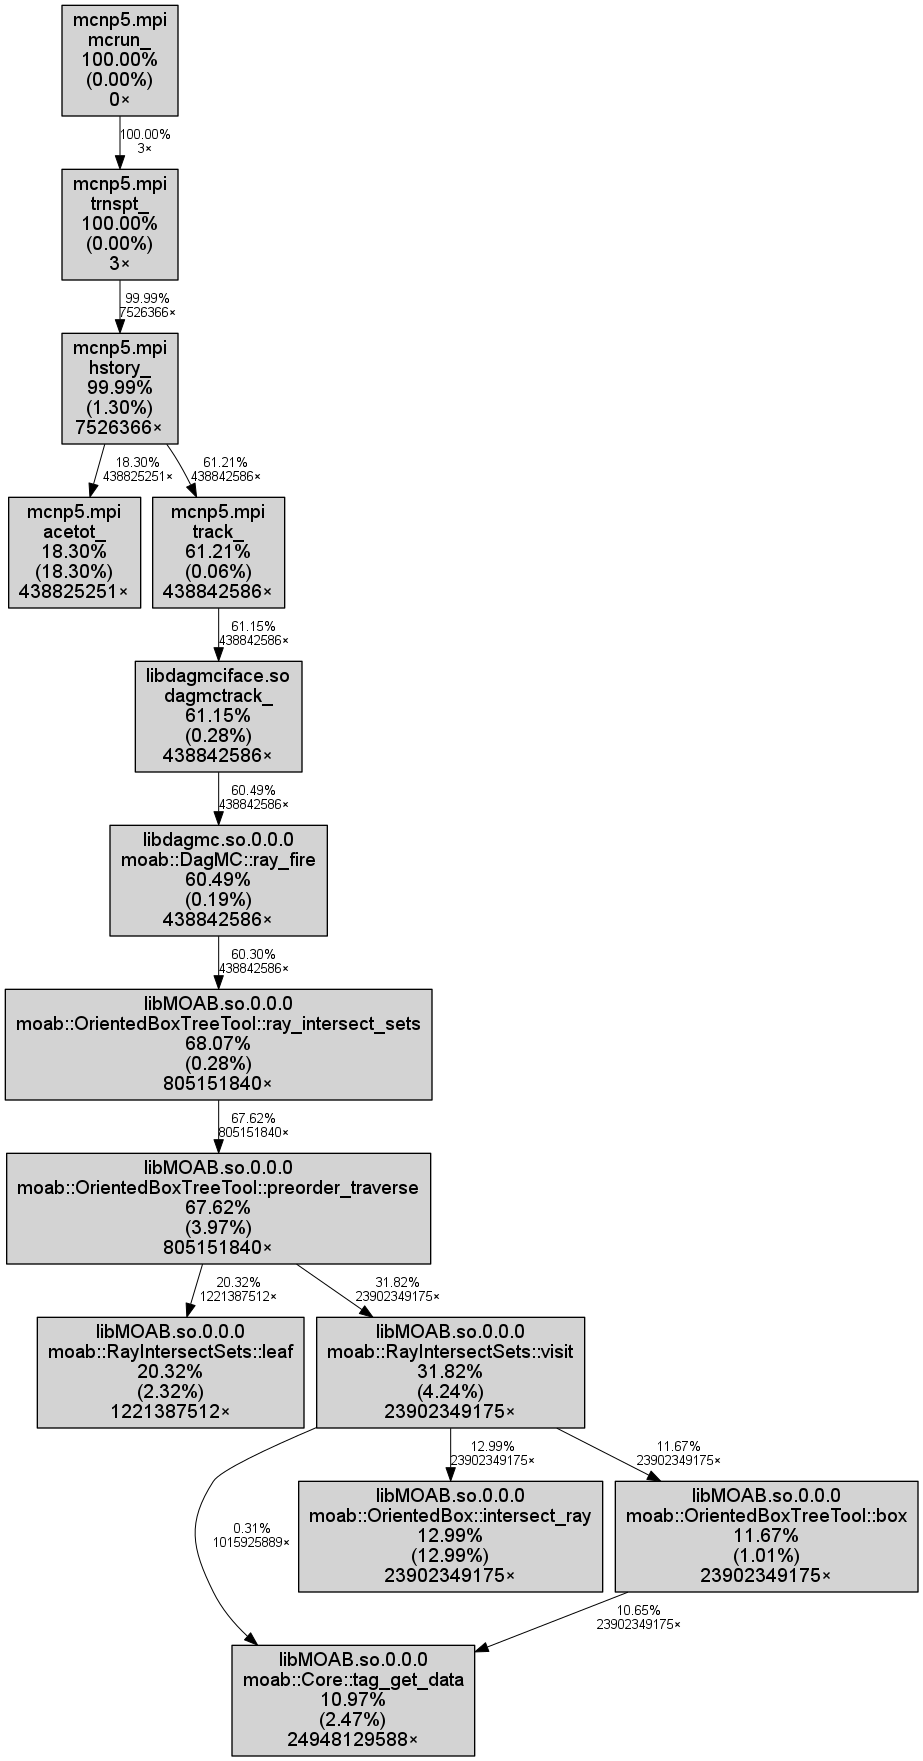
\includegraphics[scale=0.3]{dagmc_fng_cg_coarse.png}
\end{figure}

\begin{figure}[H]
  \centering
  \caption{Callgraph of native MCNP FNG run for \num{1E7} histories. Processes taking
    $<$10\% of the runtime are filtered out in order to simplify the call
    graph.}
  \label{mcnp-fng-coarse}
  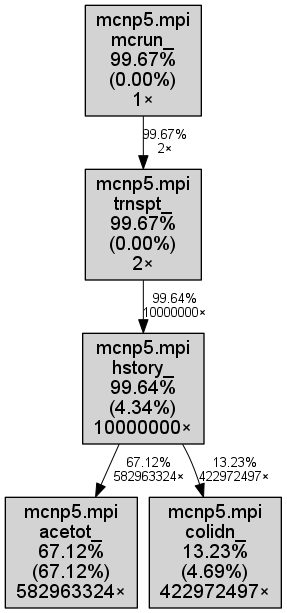
\includegraphics[scale=0.3]{native_fng_cg_coarse.png}
\end{figure}

The combination of the profiling results indicating how much time is spent in
tracking particles in DAGMC along with the difference in absolute run times
confirms that the performance bottleneck of DAGMC lies in its ability to quickly
satisfy the geometric queries of the underlying Monte Carlo code it is coupled
to. Looking more closely at the underlying calls in DAGMC, one can see that this
time is collectively spent in the DAGMC \textit{ray\_fire} method. Function names
like \textit{RayIntersectSets} and \textit{preorder\_traverse} indicate that
this time is spent in MOAB's database-oriented ray tracing implementation.

\section{Statement of Thesis}

The purpose of this dissertation is to improve the performance of CAD-based
Monte Carlo radiation transport in a manner that is widely accessible to
analysts. The result is a compilation of adaptive data structure construction,
data structure redesign, and alternative methods to reduce simulation times in
DAGMC.

A background and literature review of CAD-based transport methods and associated
acceleration techniques is provided in Chapter \ref{ch:background}. First, it
outlines required capabilities for particle tracking in MCRT. Next it describes
commonly used geometry representations in MCRT codes followed by a description
of the CAD-based particle tracking system of interest for this work. Lastly,
associated acceleration data structures and techniques which enable performant
computation of transport on CAD models are discussed.

Chapter \ref{ch:preconditioning} presents a novel acceleration method for
CAD-Based MCRT and its application for each of the relevant geometry query types
outlined in Chapter \ref{ch:background}. An analytic model is then described to
guide the application of this method based on simple parameters of the geometry
and physics of previous or partial simulations. Finally, results of this
method's application in both contrived and production models are discussed along
with limitations of the method and the aforementioned analytic model.

The integration of nuclear engineering simulation with state-of-the-art
computer graphics tools is demonstrated in Chapter \ref{ch:simd_bvh}. Significant
improvements in performance are demonstrated in both test and production models
by adapting data structures discussed in Chapter \ref{ch:background} for optimal
efficiency on modern CPU architectures. Robustness limitations of the computer graphics
tools for engineering analysis are discussed, and extensions of these tools are
presented to address those limitations. Critical implementation details and
algorithmic adjustments of these
extensions are discussed, and performance comparisons are drawn in terms of the
raw query speed between all particle tracking implementations. Finally results,
of the extended, and robust, system are presented for several production models,
including several of the models used as an initial comparison in Chapter
\ref{ch:introduction}.

Chapter \ref{ch:high_valence} addresses a long-standing issue in CAD-based
MCRT. Performance degradation caused by problematic features of the CAD-based
are characterized using a contrived model for all particle tracking
implementations found in Chapter \ref{ch:simd_bvh}. A solution using on-the-fly
detection and adaptation of this feature during construction of particle tracking
acceleration data structured is presented. Characterization of the response to
this geometric feature both with and without the adaptive construction
technique. Finally, results of this technique as applied to the same set of
production models shown in Chapter \ref{ch:simd_bvh} are presented and discussed.

The conclusion statements in Chapter \ref{ch:conclusion} discuss the
contributions of this work to MCRT for CAD geometries, its broader impacts, and
possible future directions for various aspects of the work.
